\documentclass[12 pt,a4paper]{report}

\usepackage{amstext}
\usepackage{amsfonts}
\usepackage{graphicx}
\usepackage{amssymb,amsthm,amsmath,amscd}     
\usepackage{latexsym}                         
%\usepackage{enumerate}
\usepackage[ngerman]{babel}
\usepackage[latin1]{inputenc}
\usepackage{fancyheadings}
\usepackage{float}
%\usepackage{verbatim} fuer Quelltexteingabe

\author{}
\title{}

%Befehle Block--------------------------
%\newcommand{\qed}{\hfill$\square$}
%Theorem Umgebungen---------------------

\newtheorem{thm}{\textsc{Satz}}[subsection]
\newtheorem{cor}[thm]{\textsc{Korollar}}
\newtheorem{lem}[thm]{\textsc{Lemma}}
\newtheorem{prop}[thm]{\textsc{Proposition}}

\theoremstyle{definition}
\newtheorem{defn}[thm]{\textsc{Definition}}
\newtheorem{rem}[thm]{Bemerkung}
\newtheorem{exa}[thm]{Beispiel}
\newtheorem{bez}[thm]{Bezeichnung}
\newtheorem{beh}[thm]{Behauptung}

%---------------------------------------
\pagestyle{fancy}
\rhead{}
\begin{document}
\setlength\parindent{0pt}

%Titel Seite-----------------------------
\begin{titlepage}
\begin{center}

\vspace*{1.0cm}
\huge
\textsc{\bf{Rekurrente Netze\\
		-\\
    Das Elman Netz}}

\vspace*{1.0cm}
\Large
\textsc{Bachelorarbeit}

\vspace*{4.0cm}
\textsc{
\normalsize{eingereicht von} \\[0.5\baselineskip]
{\large \ Stefan Vikoler}
}

\vspace*{3.0cm}
\textsc{
\normalsize{Betreuerin:\\
Dr. Claudia-Lidia Badea}
}

\vspace*{1.0cm}
\textsc{
\normalsize{Universit\"at Salzburg \\
Fachbereich Computerwissenschaften\\
Jakob-Haringer-Stra�e 2\\
A-5020 Salzburg\\
Austria\\
Juni 2012}
}

\end{center}

\end{titlepage}

%Include Block---------------------------
\section*{Vorwort}
\itshape
Diese Arbeit ist im Rahmen meines Bachelorabschlusses an der Universit�t Salzburg, Fachbereich Computerwissenschaften, unter der Aufsicht von Dr. Claudia-Lidia Badea entstanden. Es umfasst die Definition von rekurrenten Netzen und einen Lernalgorithmus, um rekurrente Netze zu trainieren. Hauptaugenmerk wird in dieser Arbeit auf das Elman Netz, die dynamische Backpropagation, um ein Elman Netz zu trainieren, und deren Zusammenhang mit der System Identification gelegt.\\
\upshape

Alle Abbildungen dieser Arbeit wurden, sofern nicht anders angegeben, eigenh�ndig erstellt.
\tableofcontents
\chapter{Einleitung}
\section{Architekturen von neuronalen Netzen}
Der Lernalgorithmus, mit welchem man ein Netz versucht zu trainieren, h�ngt davon ab, wie die Neuronen eines neuronalen Netzes strukturiert sind. Man kann Netz-Architekturen in drei fundamentale Klassen unterscheiden:
\begin{enumerate}
	\item Einschichtige Feedforward Netze
	\item Mehrschichtige Feedforward Netze
	\item Rekurrente Netze
\end{enumerate}

\subsection{Einschichtige Feedforward Netze}
In geschichteten neuronalen Netzen werden die Neuronen in Form von Schichten organisiert. In der einfachsten Form von geschichteten Netzen gibt es eine Input- und eine Outputschicht, wobei die Inputschicht Signale zur Outputschicht, welche die Berechnungen durchf�hrt, sendet und keine umgekehrte Verbindungen existieren. Solche Netze hei�en feedforward- oder azyklische Netze. In Abbildung \ref{single} sehen wir ein Netz mit drei Knoten in der Input- und drei Knoten in der Outputschicht. Ein solches Netz nennt man einschichtig.
\begin{figure}[H]
	\centering
	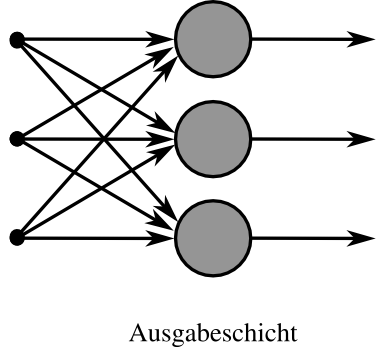
\includegraphics[height=6cm]{SingleLayer.png}
	\caption{SingleLayer Network \itshape(de.wikipedia.org)\upshape}
	\label{single}
\end{figure}

\subsection{Mehrschichtige Feedforward Netze}
Die zweite Klasse der feedforward Netze unterscheidet sich durch eine oder mehrere verdeckte Schichten, deren Knoten zur Berechnung zust�ndig sind und verdeckte Neuronen genannt werden. Ihre Aufgabe ist es, zwischen der Input- und der Outputschicht n�tzlich zu intervenieren. Abbildung \ref{multi} zeigt eine Abbildung eines mehrschichtigen feedforward Netzes mit einer einzelnen verdeckten Schicht mit 3 verdeckten Neuronen.
\begin{figure}[H]
	\centering
	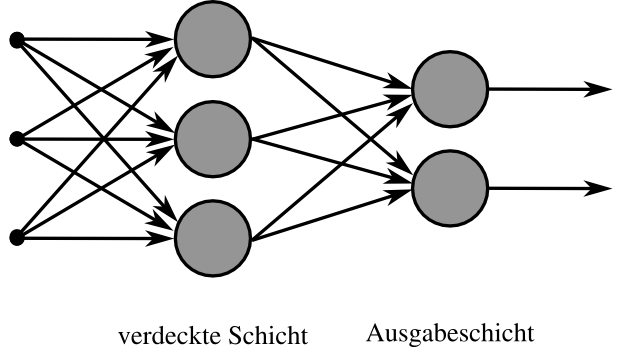
\includegraphics[height=6cm]{MultiLayer.png}
	\caption{MultiLayer Network \itshape(de.wikipedia.org)\upshape}
	\label{multi}
\end{figure}

\subsection{Rekurrente Netze}
Rekurrente Netze sind Neuronale Netze welche sich von den feedforward Netzen unterscheiden, indem sie mindestens eine umgekehrte Verbindung (R�ckkopplung) enthalten, eine sogenannte "`feedback loop"'. Zum Beispiel kann ein rekurrentes Netz (Abbildung \ref{recurrent1}) aus einer Schicht von Neuronen bestehen, welche ihr Outputsignal wieder als Inputsignal verwenden.
\begin{figure}[H]
	\centering
	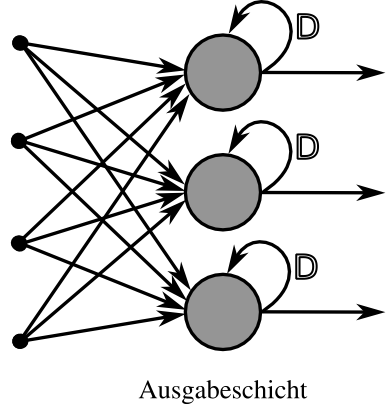
\includegraphics[height=6cm]{Recurrent.png}
	\caption{Recurrent Network 1 \itshape(de.wikipedia.org)\upshape}
	\label{recurrent1}
\end{figure}

Ein anderes Beispiel (Abbildung \ref{recurrent2}) zeigt ein rekurrentes Netz, welches das berechnete Signal der Outputschicht �ber ein zus�tzliches Neuron in der Inputschicht wieder in das Netz einspeist.
\begin{figure}[H]
	\centering
	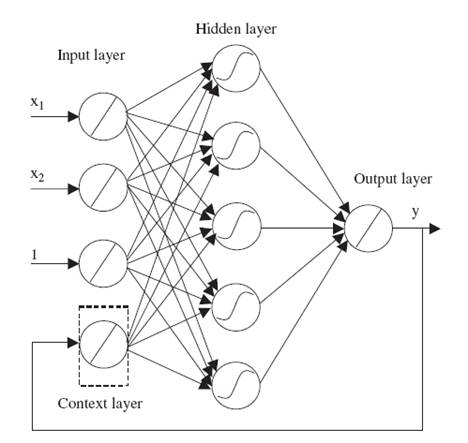
\includegraphics[height=8cm]{Recurrent2.jpg}
	\caption{Recurrent Network 2 \itshape(web.mst.edu)\upshape}
	\label{recurrent2}
\end{figure}

Die Verwendung von "`feedback loops"' hat eine nachhaltige Auswirkung auf die Lernkapazit�t und die Performanz eines Netzes. Meist werden solche umgekehrten Verbindungen zeitlich verz�gert, sodass ein Ged�chtnis und ein dynamisches Verhalten f�r das Netz entsteht.


\chapter{Rekurrente Netze}
\section{Modelle von Rekurrenten Netzen}
Wie in der Einleitung bereits erw�hnt, k�nnen die Architekturen eines rekurrenten Netzes viele verschiedene Formen annehmen. In diesem Kapitel werden zwei Modelle beschrieben, das Input-Output Model und das State-Space Model.\cite{haykin}

\subsection{Input-Output Model}
\begin{figure}[H]
	\centering
	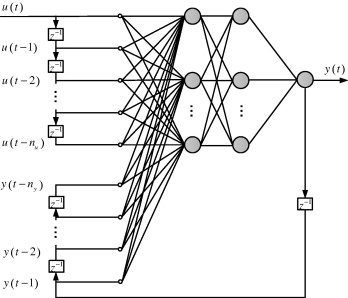
\includegraphics[height=8cm]{narx.jpg}
	\caption{Input-Output Model \itshape(sciencedirect.com)\upshape}
	\label{iomodel}
\end{figure}
Abbildung \ref{iomodel} zeigt eine Architektur eines rekurrenten Netzes mit einem einzelnen Inputsignal $u(t)$ mit einer Zeitverschiebung von $n_u$ Einheiten. Au�erdem hat es ein Outputsignal $y(t)$, welches �ber $n_y$ Zeitverschiebungen wieder als Input verwendet wird. Ein solches Modell nennt man Input-Output Model.\\
Dadurch ergeben sich folgende Inputdaten f�r das Netz:
\begin{itemize}
	\item Die akutellen und die vergangenen Inputwerte $u(t), u(t-1),\ldots,u(t-n_u)$
	\item und die zeitverz�gerten Werte des Outputneurons $y(t-1),\ldots,y(t-n_y)$.
\end{itemize}
Ein solches Modell besitzt ein dynamsiches Verhalten welches durch
$$y(t) = F\left(y(t-1),\ldots,y(t-n_y),u(t),\ldots,u(t-n_u)\right)$$
beschrieben wird, wobei $F$ eine lineare Funktion ist.

\subsection{State-Space Model}
\begin{figure}[H]
	\centering
	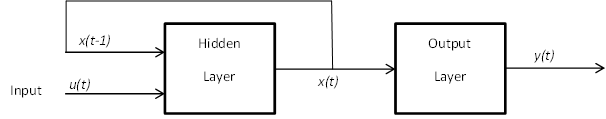
\includegraphics[width=12cm]{StateSpace.png}
	\caption{State-Space Model}
	\label{ssmodel}
\end{figure}
Abbildung \ref{ssmodel} zeigt eine weitere Architektur eines rekurrenten Netzes, welches State-Space Model genannt wird. Dabei wird der Output der verdeckten Schicht $x(t)$ zeitversetzt wieder zum Input dazugenommen. Der Input besteht also aus einer Verkettung der Inputwerte $u(t)$ und den zeitversetzten Outputwerten der verdeckten Schicht. Auch hier k�nnen mehrere zeitversetzte Werte der Input- beziehungsweise der verdeckten Schicht verwendet werden. Somit erhalten wir ein dynamisches Verhalten des State-Space Model mit der Gleichung
\begin{align*}
	x(t) &= f\left(x(t-1),u(t)\right) \text{ und}\\
	y(t) &= C x(t),
\end{align*}
wobei $f$ eine lineare Funktion und $C$ die Gewichte zur Outputschicht darstellen.\\

Beide Modelle lassen sich durch ein Elman Netz darstellen.

\chapter{Das Elman Netz}
Elman Netze\cite{elman} besitzen die Eigenschaft zeitver�nderliche Muster zu erkennen und zu klassifizieren, da bei einem Elman Netz der Output der verdeckten Schicht gespeichert und zeitversetzt als Input verwendet wird, indem man in der Inputschicht eine Kontextschicht anlegt.
\begin{figure}[H]
	\centering
	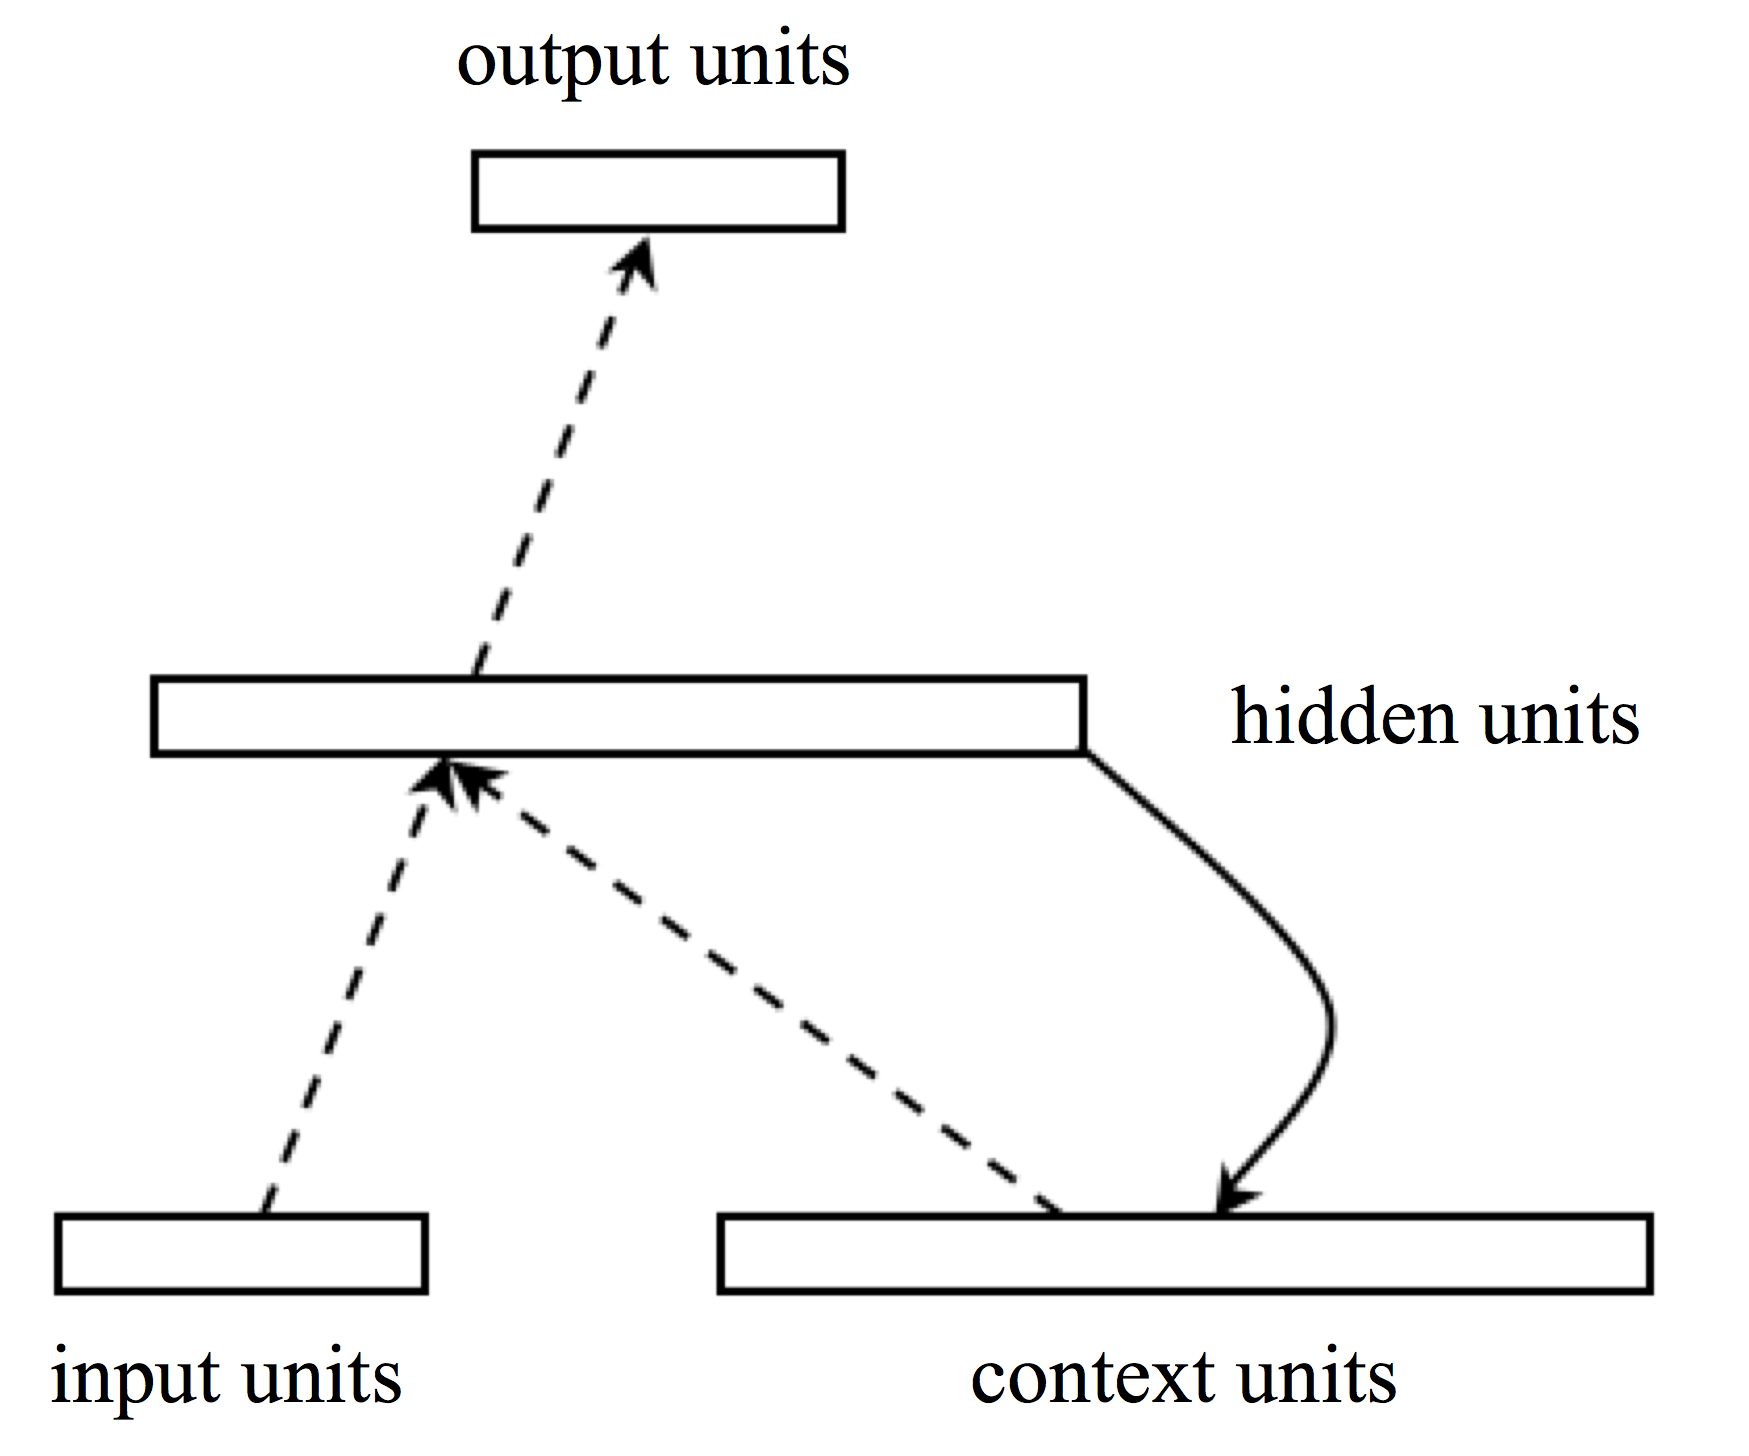
\includegraphics[height=6cm]{elman.png}
	\caption{Elman Network\itshape(plato.stanford.edu)\upshape}
	\label{elmanNet}
\end{figure}
Die Architektur (Abbildung \ref{elmanNet}) eines Elman Netzes besteht also aus einer Inputschicht, einer verdeckten Schicht, einer Outputschicht und der Kontextschicht, in der die Werte der verdeckten Schicht zeitversetzt gespeichert werden. Somit wird der innere Zustand des Netzes in der Kontextschicht gespeichert.
\chapter{Der Algorithmus}
Es existieren verschiedenste Lernalgorithmen um Elman Netze und im Allgemeinen rekurrente Netze zu trainieren. Vieles h�ngt von der Architektur und der Aufgabenstellung des Netzes ab. Beispiele sind etwa 
\begin{itemize}
	\item der dynamische Backpropagation Algorithmus,
	\item der Real-Time Recurrent Learning Algorithmus
	\item oder die Kalman Filter.
\end{itemize}
In dieser Arbeit wird speziell auf den dynamischen Backpropagation Algorithmus\cite{pham} eingegangen.

\section{Dynamische Backpropagation}
\begin{figure}[H]
	\centering
	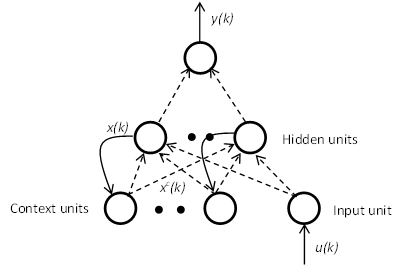
\includegraphics[height=6cm]{BasicElman.png}
	\caption{Basic Elman Network}
	\label{basicElman}
\end{figure}
Abbildung \ref{basicElman} zeigt die Architektur eines klassischen Elman Netzes nach Elman 1990\cite{elman}. Die feedforward-Verbindungen (gestrichelte Linien) sind ver�nderbar und die rekurrenten Verbindungen (geschlossene Linien) sind fix.

\subsection{Berechnung der Neuronen}
Sei der Input des Netzes $u(k)$, der Output $y(k)$, der gesamte Input zu den einem $i$-ten verdeckten Neuron $v_i(k)$, der Output eines $i$-ten verdeckten Neuron $x_i(k)$ und der Output eines $j$-ten Kontextneurons $x_j^c(k)$, dann gilt:
\begin{align}
	v_i(k) &= \sum\limits_{j=1}^n w_{i,j}^x(k-1) x_j^c(k) + w_i^u(k-1) u(k), \tag{1a}\\
	x_i(k) &= f(v_i), \tag{1b}\\
	x_j^c(k) &= x_j(k-1), \tag{1c}\\
	y(k) &= \sum\limits_{i=1}^n w_i^y(k-1) x_i(k), \tag{1d}
\end{align}
wobei $w_i^u, w_{i,j}^x$ und $w_i^y$, $i,j=1,\ldots,n$, die Gewichte der Verbindungen zwischen Input- und verdeckter Schicht, Kontext- und verdeckter Schicht und zwischen verdeckter und Outputschicht sind und $f$ eine sigmoidale Aktivierungsfunktion ist.

Wird nun der Input $u(k)$ um einen Zeitschritt verz�gert, bevor er gesendet wird, wird $x_j^c(k)$ mit $x_j(k-1)$ ersetzt und angenommen die verdeckten Neuronen sind linear, dann gelten folgende Gleichungen:
\begin{align}
	v_i(k) &= \sum\limits_{j=1}^n w_{i,j}^x(k-1) x_j(k-1) + w_i^u(k-1) u(k-1), \tag{2a}\\
	x_i(k) &= v_i(k), \tag{2b}\\
	y(k) &= \sum\limits_{i=1}^n w_i^y(k-1) x_i(k). \tag{2c}
\end{align}
Diese Gleichungen beschreiben ein State-Space Model $n$-ter Ordnung eines linearen dynamischen Systems und k�nnen als folgende Gleichung dargestellt werden:
\begin{align}
	y(k) &= A_1 y(k-1) + A_2 y(k-2) + \cdots + A_n y(k-n) \notag \\
	&+ B_1 u(k-1) + B_2 u(k-2) + \cdots + B_n u(k-n). \tag{3}
\end{align}

\subsection{Training durch dynamische Backpropagation}
Seien die Trainingswerte das Paar $(u(k),y_d(k))$, $k=1,2,\ldots,N$, mit $u(k)$ als Input und $y_d(k)$ als gew�nschter Output.\\
Die Fehlerfunktion des Netzes zum Zeitpunkt $k$ ist
\begin{align}
	E_k = \frac{1}{2} \left(y_d(k)-y(k)\right)^2. \tag{4}
\end{align}
Die Gewichte des Netzes werden zu jedem Zeitpunkt $k$ modifiziert. Der Fehlergradient f�r $w_i^y(k-1)$ ist
\begin{align}
	\frac{\partial E_k}{\partial w_i^y(k-1)} &= -(y_d(k)-y(k)) \frac{\partial y(k)}{\partial w_i^y(k-1)} \notag \\
	&= -(y_d(k)-y(k)) x_i(k). \tag{5}
\end{align}
Die Fehlergradienten f�r $w_i^u(k-1)$ und $w_{i,j}^x(k-1)$ lauten
\begin{align}
	\frac{\partial E_k}{\partial w_i^u(k-1)} &= -\frac{\partial E_k}{\partial y(k)} \frac{\partial y(k)}{\partial x_i(k)} \frac{\partial x_i(k)}{\partial v_i(k)} \frac{\partial v_i(k)}{\partial w_i^u(k-1)} \notag \\
	&= -(y_d(k)-y(k)) w_i^y(k-1) f'(u(k)) \tag{6}
\end{align}
und
\begin{align}
	\frac{\partial E_k}{\partial w_{i,j}^x(k-1)} &= -\frac{\partial E_k}{\partial y(k)} \frac{\partial y(k)}{\partial x_i(k)} \frac{\partial x_i(k)}{\partial w_{i,j}^x(k-1)} \notag \\
	&= -(y_d(k)-y(k)) w_i^y(k-1) \frac{\partial x_i(k)}{\partial w_{i,j}^x(k-1)}, \tag{7}
\end{align}
wobei
\begin{align}
	\frac{\partial x_i(k)}{\partial w_{i,j}^x(k-1)} &= \frac{\partial x_i(k)}{\partial v_i(k)} \frac{\partial v_i(k)}{\partial w_{i,j}^x(k-1)} \notag \\
	&= f'\left(\frac{\partial v_i(k)}{\partial w_{i,j}^x(k-1)}\right) \notag \\
	&= f'\left(x_j(k-1) + \sum\limits_{l=1}^n w_{i,l}^x(k-1) \frac{\partial x_l(k-1)}{\partial w_{i,j}^x(k-2)}\right). \tag{8}
\end{align}

\subsection{Zusammenfassung}
Der dynamische Backpropagation-Algorithmus kann nun wie folgt zusammengefasst werden.\\
\subsubsection{Berechnung der Neuronen:}
\begin{align}
	v_i(k) &= \sum\limits_{j=1}^n w_{i,j}^x(k-1) x_j(k-1) + w_i^u(k-1) u(k), \tag{9a} \\
	x_i(k) &= f(v_i), \tag{9b} \\
	y(k) &= \sum\limits_{i=1}^n w_i^y(k-1) x_i(k). \tag{9c}
\end{align}
\subsubsection{Update der Gewichte:}
\begin{align}
	w_i^y(k) &= w_i^y(k-1) - \eta (y_d(k)-y(k)) x_i(k), \tag{10a} \\
	w_i^u(k) &= w_i^u(k-1) - \eta (y_d(k)-y(k)) w_i^y(k-1) f'(u(k)), \tag{10b} \\
	w_{i,j}^x(k) &= w_{i,j}^x(k-1) - \eta (y_d(k)-y(k)) w_i^y(k-1) \frac{\partial x_i(k)}{\partial w_{i,j}^x(k-1)}, \tag{10c} \\
	\frac{\partial x_i(k)}{\partial w_{i,j}^x(k-1)} &= f'\left(x_j(k-1) + \sum\limits_{l=1}^n w_{i,l}^x(k-1) \frac{\partial x_l(k-1)}{\partial w_{i,j}^x(k-2)}\right). \tag{10d}
\end{align}

\chapter{Anwendungen}
In dieser Arbeit werden zwei Anwendungen eines Elman Netzes vorgestellt. Zum Einen eine klassische Aufgabenstellung f�r solche Netze, die System Identification eines Input-Output Model und zum Anderen eine ungew�hnliche Problematik f�r Elman Netze, die Approximation von Funktionen.

\section{System Identification}
System Identification\cite{haykin} ist die experimentelle Ann�herung, um einen Prozess oder eine Anlage mit unbekannten Parametern zu modellieren. Dazu werden folgende Schritte ben�tigt:
\begin{itemize}
	\item Experimentelles Planen
	\item Auswahl einer Modellstruktur
	\item Sch�tzung der Parameter
	\item Modellauswertung
\end{itemize}
Der Prozess der System Identification ist iterativ, in dem man Schritte zur�ck und wieder vorw�rts gehen muss, bis ein zufriedenstellendes Modell erzeugt wurde.
Bei der System Identification haben wir die Wahl zwischen einem State-Space Model oder einem Input-Output Model.

\subsection{System Identification eines Input-Output Model}
Angenommen der unbekannte Prozess ist nur �ber seinen Output erreichbar.\\
Seien $u(t)$ der externe Input und $y(t)$ der Netzoutput zum Zeitschritt $t$ und das Input-Output Model wie folgt:
$$y(t) = a_1 y(t-2) + a_2 y(t-2) + a_3 y(t-3) + b_1 u(t-1),$$
wobei $a_1 = 2.627771, a_2 = -2.333261, a_3 = 0.697676, b_1 = 0.017203$.

Danach w�hle ich meine Architektur wie folgt:
\begin{figure}[H]
	\centering
	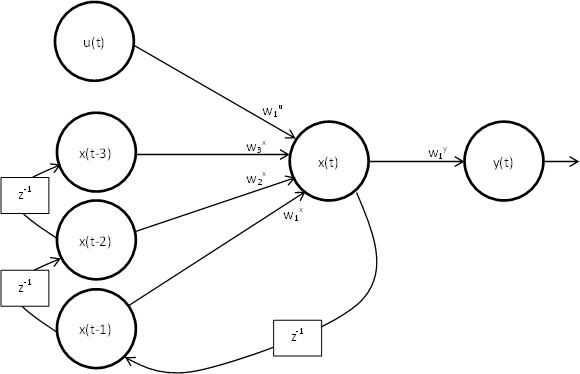
\includegraphics[height=7cm]{architektur2.png}
	\caption{Architektur}
	\label{arche}
\end{figure}

Abbildung \ref{arche} zeigt eine Architektur mit 
\begin{itemize}
	\item einem Inputneuron $u(t)$,
	\item einem verdeckten Neuron $x(t)$,
	\item einem Outputneuron $y(t)$
	\item und drei Kontextneuronen $x(t-1), x(t-2), x(t-3)$
\end{itemize}
mit den dazugeh�rigen Gewichten. Wobei $w_1^u$ das Gewicht der Verbindung vom Inputneuron zum verdeckten Neuron, $w_i^x$, $1 \leq i \leq 3$, die Gewichte von der Kontextschicht zum verdeckten Neuron und $w_1^y$ das Gewicht vom verdeckten Neuron zum Outputneuron darstellen. $z^{-1}$ stellt den Shiftoperator dar, welcher den Wert der Verbindung um einen Zeitschitt verz�gert. Weiters wird als Lernparameter $\eta = 0,7$ und als Aktivierungsfunktion die Sigmoide (Abbildung \ref{sigmoid}) verwendet:
$$\varphi(x) = \frac{1}{1+e^{-x}}$$
\begin{figure}[H]
	\centering
	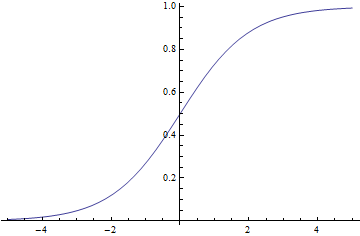
\includegraphics[height=6cm]{sigmoid.png}
	\caption{Sigmoide}
	\label{sigmoid}
\end{figure}

Dieses Netz kann man nun mit dem dynamischen Backpropagation Algorithmus sehr erfolgreich trainieren. Dazu werden 100 Input- und Outputwerte verwendet und es sind folgende Berechnungen pro Zeitschitt n�tig:
\begin{align*}
	v(t) &= w_1^x x(t-1) + w_2^x x(t-2) + w_3^x x(t-3) + w_1^u u(t) \\
	x(t) &= \varphi(v) \\
	y(t) &= w_1^y x(t)
\end{align*}
\begin{align*}
	w_1^u(t) &= w_1^u(t-1) - \eta (y_d(t)-y(t)) w_1^y(t-1) \varphi'(u(t)) \\
	w_1^x(t) &= w_1^x(t-1) - \eta (y_d(t)-y(t)) w_1^y(t-1) \frac{\partial x(t)}{\partial w_1^x(t-1)} \\
	w_2^x(t) &= w_2^x(t-1) - \eta (y_d(t)-y(t)) w_1^y(t-1) \frac{\partial x(t)}{\partial w_2^x(t-1)} \\
	w_3^x(t) &= w_3^x(t-1) - \eta (y_d(t)-y(t)) w_1^y(t-1) \frac{\partial x(t)}{\partial w_3^x(t-1)} \\
	w_1^y(t) &= w_1^y(t-1) - \eta (y_d(t)-y(t)) x(t)
\end{align*}

Ein so trainiertes Elman Netz liefert zum obigen Input-Output Model und nach 100 Epochen folgendes Ergebnis (Abbildung \ref{result1}), wobei die blaue Linie das anzun�hernde Input-Output Model und die violetten Punkte den Netzoutput darstellen.
\begin{figure}[H]
	\centering
	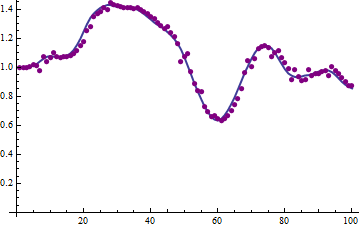
\includegraphics[height=7cm]{Plot1.png}
	\caption{System Identification}
	\label{result1}
\end{figure}

Zu beachten ist, dass durch die Wahl einer anderen Architektur oder bei einem zu niedrig gew�hlten Lernparameter die Ergebnisse trotz dynamischer Backpropagation abweichen k�nnen. Dies zeigt Abbildung \ref{result2}.
\begin{figure}[H]
	\centering
	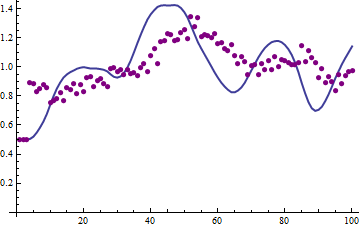
\includegraphics[height=6cm]{Plot2.png}
	\caption{Fehlerdarstellung}
	\label{result2}
\end{figure}

\section{Approximation von Funktionen}
Da die Approximation von Funktionen nicht zu den gew�hnlichen Aufgaben eines Elman Netzes geh�rt, habe ich versucht eine Funktion mit dem selben Netz, welches bei der System Identification verwendet wurde, zu approximieren. Das hei�t, es wurde die selbe Architektur (Abbildung \ref{arche}), der selbe Lernparameter $\eta = 0,7$, die selbe Aktivierungsfunktion $\varphi(x) = \frac{1}{1+e^{-x}}$ und die gleich Menge an 100 Input- und Outputwerten verwendet. Als die zu approximierende Funktion w�hlte ich
$$e^{-\frac{x}{4}} \cos x.$$
Diese Funktion wird in Abbildung \ref{function} dargestellt.
\begin{figure}[H]
	\centering
	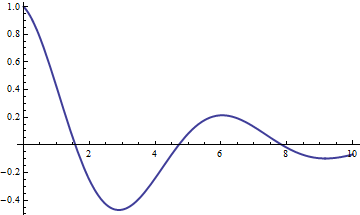
\includegraphics[height=6cm]{func.png}
	\caption{Funktion}
	\label{function}
\end{figure} 

Nach 100 Epochen meines Netzes erhalte ich folgende Gegen�berstellung (Abbildung \ref{result3}), wobei die blaue Linie die zu approximierende Funktion und die violetten Punkte den Netzoutput darstellen.
\begin{figure}[H]
	\centering
	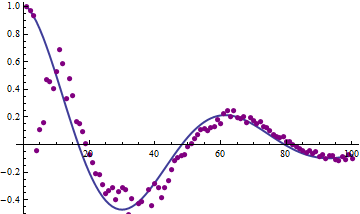
\includegraphics[height=6cm]{approx.png}
	\caption{Approximation}
	\label{result3}
\end{figure}

\section{Fazit}
Wie die Gegen�berstellung zeigt, ist die Approximation noch nicht ausgereift und man kann mit einer anderen Architektur eventuell bessere Werte erzielen. Au�erdem ist diese Gegen�berstellung ein Ausnahmebeispiel meines Netzes und nicht alle 100 Epochen wurden so gute Ergebnisse getroffen. Der Gesamtfehler liegt hier bei $E = 1,3207026786535492$, wobei der Gesamtfehler der System Identification unter $0,2$ liegt. Abschlie�end kann man sagen, dass das Problem der System Identification mittels der durch die dynamische Backpropagation trainierten Elman Netze gute Ergebnisse erzielt und f�r die Funktionenapproximation gr��ere Fehler aufweist.

\chapter*{Abbildungsverzeichnis}

\begin{tabbing}
	\hspace*{0.5cm}\=\hspace*{4.2cm}\=\hspace*{3cm}\=\hspace*{5cm}\= \kill
	\>{\bf Abbildung} \> {\bf } \> {\bf } \> {\bf Seite} \\ \ \\
	\>Abb. \ref{single}: SingleLayer Network \itshape(de.wikipedia.org)\upshape \> \> \> \pageref{single} \\ \ \\
	\>Abb. \ref{multi}: MultiLayer Network \itshape(de.wikipedia.org)\upshape \> \> \> \pageref{multi} \\ \ \\
	\>Abb. \ref{recurrent1}: Recurrent Network 1 \itshape(de.wikipedia.org)\upshape \> \> \> \pageref{recurrent1} \\ \ \\
	\>Abb. \ref{recurrent2}: Recurrent Network 2 \itshape(web.mst.edu)\upshape \> \> \> \pageref{recurrent2} \\ \ \\
	\>Abb. \ref{iomodel}: Input-Output Model \itshape(sciencedirect.com)\upshape \> \> \> \pageref{iomodel} \\ \ \\
	\>Abb. \ref{ssmodel}: State-Space Model \> \> \> \pageref{ssmodel} \\ \ \\
	\>Abb. \ref{elmanNet}: Elman Network\itshape(plato.stanford.edu)\upshape \> \> \> \pageref{elmanNet} \\ \ \\
	\>Abb. \ref{basicElman}: Basic Elman Network \> \> \> \pageref{basicElman} \\ \ \\
	\>Abb. \ref{arche}: Architektur \> \> \> \pageref{arche} \\ \ \\
	\>Abb. \ref{sigmoid}: Sigmoide \> \> \> \pageref{sigmoid} \\ \ \\
	\>Abb. \ref{result1}: System Identification \> \> \> \pageref{result1} \\ \ \\
	\>Abb. \ref{result2}: Fehlerdarstellung \> \> \> \pageref{result2} \\ \ \\
	\>Abb. \ref{function}: Funktion \> \> \> \pageref{function} \\ \ \\
	\>Abb. \ref{result3}: Approximation \> \> \> \pageref{result3} \\ \ \\
\end{tabbing}
%\listoffigures

%----------------------------------------
\bibliographystyle{plain}
\nocite{*}
\bibliography{literatur}
%----------------------------------------
\end{document}